\documentclass[11pt,letterpaper]{article}
\usepackage[top=3cm, bottom=2cm, left=2cm, right=2cm, columnsep=20pt]{geometry}
\usepackage{pdfpages}
\usepackage{graphicx}
\usepackage{etoolbox}
\apptocmd{\sloppy}{\hbadness 10000\relax}{}{}
% \usepackage[numbers]{natbib}
\usepackage[T1]{fontenc}
\usepackage{ragged2e}
\usepackage[french]{babel}
\usepackage{listings}
\usepackage{color}
\usepackage{soul}
\usepackage[utf8]{inputenc}
\usepackage[export]{adjustbox}
\usepackage{caption}
\usepackage{amsmath}
\usepackage{amssymb}
\usepackage{float}
\usepackage{csquotes}
\usepackage{fancyhdr}
\usepackage{wallpaper}
\usepackage{siunitx}
\usepackage[indent]{parskip}
\usepackage{textcomp}
\usepackage{gensymb}
\usepackage{multirow}
\usepackage[hidelinks]{hyperref}
\usepackage{abstract}
\renewcommand{\abstractnamefont}{\normalfont\bfseries}
\renewcommand{\abstracttextfont}{\normalfont\itshape}
\usepackage{titlesec}
\titleformat{\section}{\large\bfseries}{\thesection}{1em}{}
\titleformat{\subsection}{\normalsize\bfseries}{\thesubsection}{1em}{}
\titleformat{\subsubsection}{\normalsize\bfseries}{\thesubsubsection}{1em}{}

\usepackage{xcolor}
\definecolor{codegreen}{rgb}{0,0.6,0}
\definecolor{codegray}{rgb}{0.5,0.5,0.5}
\definecolor{codepurple}{rgb}{0.58,0,0.82}
\definecolor{backcolour}{rgb}{0.95,0.95,0.92}
\lstdefinestyle{mystyle}{
    backgroundcolor=\color{backcolour},   
    commentstyle=\color{codegreen},
    keywordstyle=\color{magenta},
    numberstyle=\tiny\color{codegray},
    stringstyle=\color{codepurple},
    basicstyle=\ttfamily\footnotesize,
    breakatwhitespace=false,         
    breaklines=true,                 
    captionpos=b,                    
    keepspaces=true,                 
    numbers=left,                    
    numbersep=5pt,                  
    showspaces=false,                
    showstringspaces=false,
    showtabs=false,                  
    tabsize=2
}
\lstset{style=mystyle}

\usepackage[most]{tcolorbox}
\newtcolorbox{note}[1][]{
  enhanced jigsaw,
  borderline west={2pt}{0pt}{black},
  sharp corners,
  boxrule=0pt, 
  fonttitle={\large\bfseries},
  coltitle={black},
  title={Note:\ },
  attach title to upper,
  #1
}

%----------------------------------------------------

\setlength{\parindent}{0pt}
\DeclareCaptionLabelFormat{mycaptionlabel}{#1 #2}
\captionsetup[figure]{labelsep=colon}
\captionsetup{labelformat=mycaptionlabel}
\captionsetup[figure]{name={Figure }}
\newcommand{\inlinecode}{\normalfont\texttt}
\usepackage{enumitem}
\setlist[itemize]{label=\textbullet}

\begin{document}
\begin{titlepage}
\center

\begin{figure}
    \ThisULCornerWallPaper{.4}{Polytechnique_signature-RGB-gauche_FR.png}
\end{figure}
\vspace*{2 cm}

\textsc{\Large \textbf{PHS2223 --} Introduction à l'optique moderne}\\[0.5cm]
\large{\textbf{Équipe : 04}}\\[1.5cm]

\rule{\linewidth}{0.5mm} \\[0.5cm]
\Large{\textbf{Expérience 3}} \\[0.2cm]
\text{Mesure de polarisation}\\
\rule{\linewidth}{0.2mm} \\[2.3cm]

\large{\textbf{Présenté à}\\
  Guillaume Sheehy\\
  Esmat Zamani\\[2.5cm]
  \textbf{Par :}\\
  Émile \textbf{Guertin-Picard} (2208363)\\
  Laura-Li \textbf{Gilbert} (2204234)\\
  Tom \textbf{Dessauvages} (2133573)\\[3cm]}

\large{\today\\
Département de Génie Physique\\
Polytechnique Montréal\\}

\end{titlepage}

%----------------------------------------------------

\tableofcontents
\pagenumbering{roman}
\newpage

\pagestyle{fancy}
\setlength{\headheight}{14pt}
\renewcommand{\headrulewidth}{0pt}
\fancyfoot[R]{\thepage}

\pagestyle{fancy}
\fancyhf{}
\renewcommand{\headrulewidth}{1pt}
\fancyhead[L]{\textbf{PHS2223}}
\fancyhead[C]{Mesure de polarisation}
\fancyhead[R]{\today}
\fancyfoot[R]{\thepage}

\pagenumbering{arabic}
\setcounter{page}{1}

%----------------------------------------------------

\section{Résultats}

Suite à la prise de données au laboratoire, il est possible de comparer les valeurs de
coefficients de transmission obtenus aux hypothèses émises pour les mesures à deux et trois polariseurs.
En reprenant la courbe proportionnelle à $\cos^{2}\left( \theta \right)$ pour le montage de
deux polariseurs, la figure \ref{2pol} montre les valeurs obtenues, qui suivent très bien la
tendance prédite.

\begin{figure}[H]
  \centering
  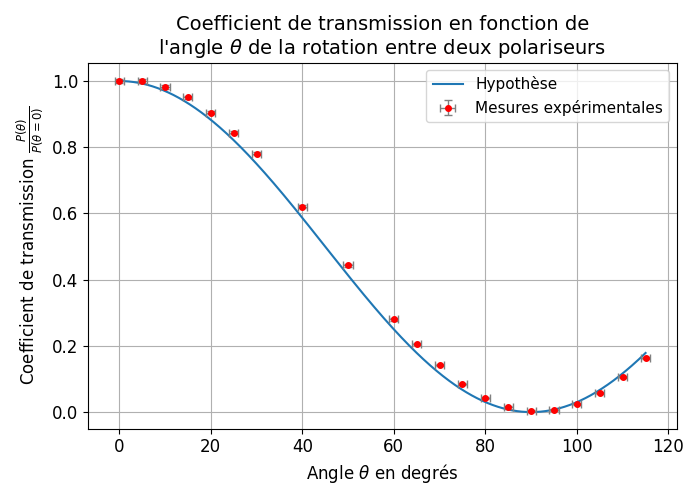
\includegraphics[scale=0.7]{viz_deux_pol.png}
  \caption{Résultats de la prise de mesure superposée à la prédiction de l'hypothèse pour la 
  mesure à deux polariseurs.}
  \label{2pol}
\end{figure}

De même pour le montage à trois polariseurs, la figure \ref{3pol} montre les valeurs de coefficient
de transmission expérimentales, qui suivent aussi bien la courbe proportionnelle à 
$\cos^{4}\left( \theta \right)$ émise par l'hypothèse.

\begin{figure}[H]
  \centering
  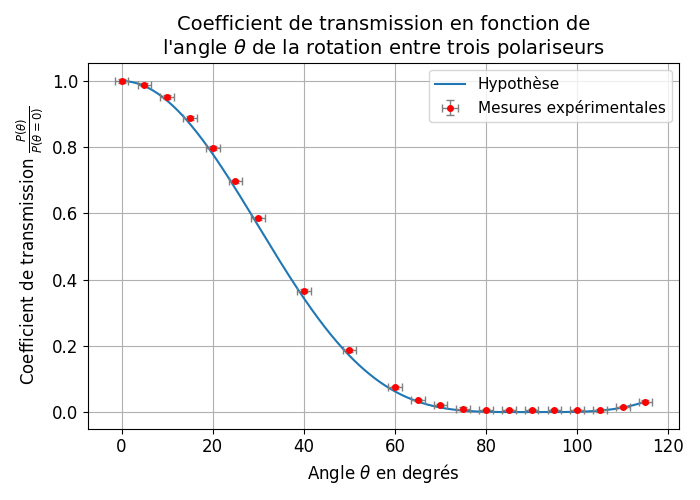
\includegraphics[scale=0.7]{viz_trois_pol.png}
  \caption{Résultats de la prise de mesure superposée à la prédiction de l'hypothèse pour la 
  mesure à trois polariseurs.}
  \label{3pol}
\end{figure}

\subsection{Estimation des erreurs}

Les incertitudes présentées avec les barres d'erreurs dans les graphiques ont été trouvées comme suit.
Pour les incertitudes sur l'angle $\theta$, la valeur est tout simplement la moitié de la plus petite
graduation sur les cadrans gradués, multiplié par le nombre de cadrans utilisés. Ainsi, pour les
mesures à deux polariseurs, comme la plus petite graduation était de $1\degree$, l'incertitude 
$\Delta\theta$  sur l'angle est aussi de $1\degree$. Pour trois polariseurs, $\Delta\theta = 1.5\degree$. 

Pour les incertitudes sur les coefficients de transmission $C$, dont le calcul se fait par

\begin{equation}
  C = \frac{P}{P_{0}},
\end{equation}

où $P$ est la puissance mesurée à un certain angle $\theta$ et $P_{0}$ est $P\left( \theta= 0 \right)$.
La propagation d'erreur pour une division de la sorte permet de calculer l'incertitude sur $C$ pour un
certain $P$ \textcolor{red}{source A} :

\begin{equation}
  \Delta C = C\sqrt{\left( \frac{\Delta P}{P} \right)^{2} + \left( \frac{\Delta P_{0}}{P_{0}} \right)^{2}},
\end{equation}

où $\Delta P$ et $\Delta P_{0}$ sont des incertitudes correspondant à la plus petite valeur lisible au
compteur de puissance, qui valent tous les deux $0.001$ mW. Selon le modèle mathématique de 
l'erreur $\Delta C$ et selon les données expérimentales, il est possible de voir que l'erreur maximale 
est en $\theta= 0$ où $C$ est maximal. Ainsi, en remplaçant par les valeurs numériques obtenues lors 
des expériences, il est possible d'estimer l'erreur sur les ordonnées en posant une borne supérieure 
sur la valeur qu'elle peut prendre :

\begin{align*}
  \text{Deux polariseurs : }\Delta C &\leq 0.005\\ 
  \text{Trois polariseurs : }\Delta C &\leq 0.008
\end{align*}

Les erreurs relatives maximales, étant donné que les coefficients à l'angle $\theta= 0$ sont donc de 0.5\% et de 0.8\% pour deux et trois polariseurs, ce qui est faible et signe d'un résultat avec une bonne exactitude.
% Source A : https://chem.libretexts.org/Bookshelves/Analytical_Chemistry/Supplemental_Modules_(Analytical_Chemistry)/Quantifying_Nature/Significant_Digits/Propagation_of_Error

\section{Discussion}

\subsection{Analyse des causes d'erreurs}

\subsection{Discussion sur les modèles}

\subsection{Question 1}

\subsection{Question 2}

\subsection{Question 3}

\subsection{Question 4}

\section{Conclusion}



\clearpage

% \bibliographystyle{unsrtnat}
% \bibliography{My_Library}

\end{document}
